%%%%% Beginning of preamble %%%%%

\documentclass[12pt]{article}  %What kind of document (article) and what size
\usepackage[document]{ragged2e}


%Packages to load which give you useful commands
\usepackage{graphicx}
\usepackage{amssymb, amsmath, amsthm}
\usepackage{fancyhdr}
\usepackage[linguistics]{forest}
\usepackage{enumerate}
\usepackage[margin=1in]{geometry} 
\pagestyle{fancy}
\fancyhf{}
\lhead{MA 750: Project 1}
\rhead{Benjamin Draves}


\renewcommand{\headrulewidth}{.4pt}
\renewcommand{\footrulewidth}{0.4pt}


\topmargin = -0.4 in
\parskip = 0.2in

%%%%%%%%%%new commands%%%%%%%%%%%%
\newcommand{\N}{{\mathbb{N}}}
\newcommand{\Z}{{\mathbb{Z}}}
\newcommand{\R}{{\mathbb{R}}}
\newcommand{\Q}{{\mathbb{Q}}}
\newcommand{\e}{{\epsilon}}
\newcommand{\del}{{\delta}}
\newcommand{\m}{{\mid}}
\newcommand{\infsum}{{\sum_{n=1}^\infty}}
\newcommand{\la}{{\langle}}
\newcommand{\ra}{{\rangle}}
\newcommand{\E}{{\mathbb{E}}}
\newcommand{\V}{{\mathbb{V}}}

%defines a few theorem-type environments
\newtheorem{theorem}{Theorem}
\newtheorem{corollary}[theorem]{Corollary}
\newtheorem{definition}{Definition}
\newtheorem{lemma}[theorem]{Lemma}
%%%%% End of preamble %%%%%

\begin{document}

\begin{enumerate}

\item \begin{enumerate}

\item We begin implementation procedures by assuming that $K$ is a Gaussian kernel and our initial estimate of the density, $\widetilde{f}$, is the density estimate from the normal kernel with the rule of thumb bandwidth ($\hat{h} = 1.06\hat{\sigma}n^{-1/n}$). Since our estimate of $\widetilde{f}$ will change, the functionality to change these assumptions is included. The function \textit{f\_var\_bw} has four arguments - $X$ the data, $k$ the name of the kernel to be used for $\widetilde{f}$, $bw$ the bandwidth to be used for $\widetilde{f}$, and $h$ the bandwidth for the estimation of $f$. For details, see the code that is attached. 

\item After successfully implementing the procedure, we looked to find a reasonable value for $h$. We began by searching over the candidate grid $\mathcal{H} = \{0.05, 0.1, 0.15, 0.25, 0.3\}$. The density estimates associated with these bandwidths are given in the figure below. 

\begin{figure}[h]
\centering
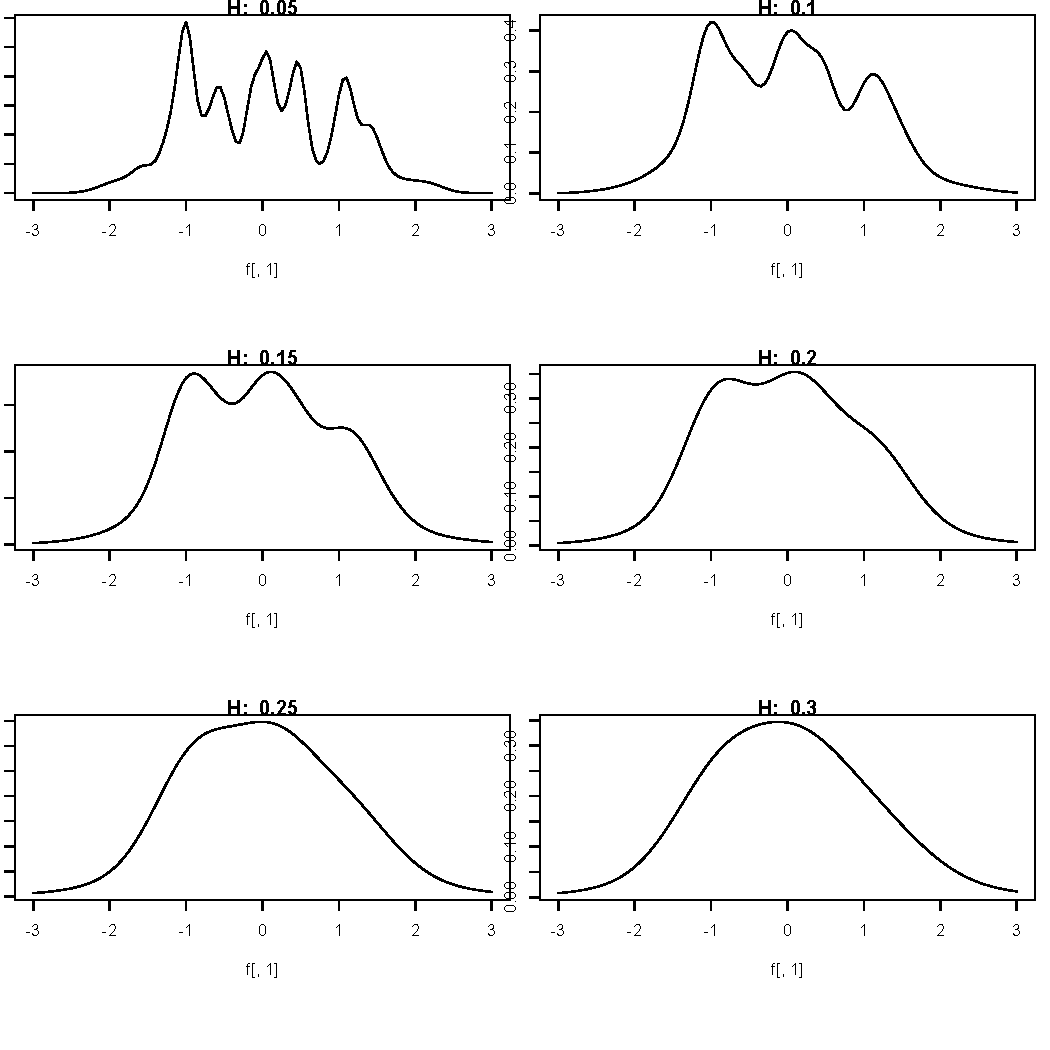
\includegraphics[width = 0.6\textwidth]{p1.pdf}
\end{figure}

It appears that for $h>0.2$ we over smooth and suppress underling modes in the data. For $h = 0.05$ it looks like the density is under smoothed with many sharp turns. For $0.05<h\leq 0.2$ is is hard to determine which bandwidth offers optimal smoothing. For this reason, we reduce our search to $\mathcal{H} =\{0.1,0.12, 0.14, 0.16, 0.18, 0.2\}$ The plots of these kernel estimate is given below.

\begin{figure}[h]
\centering
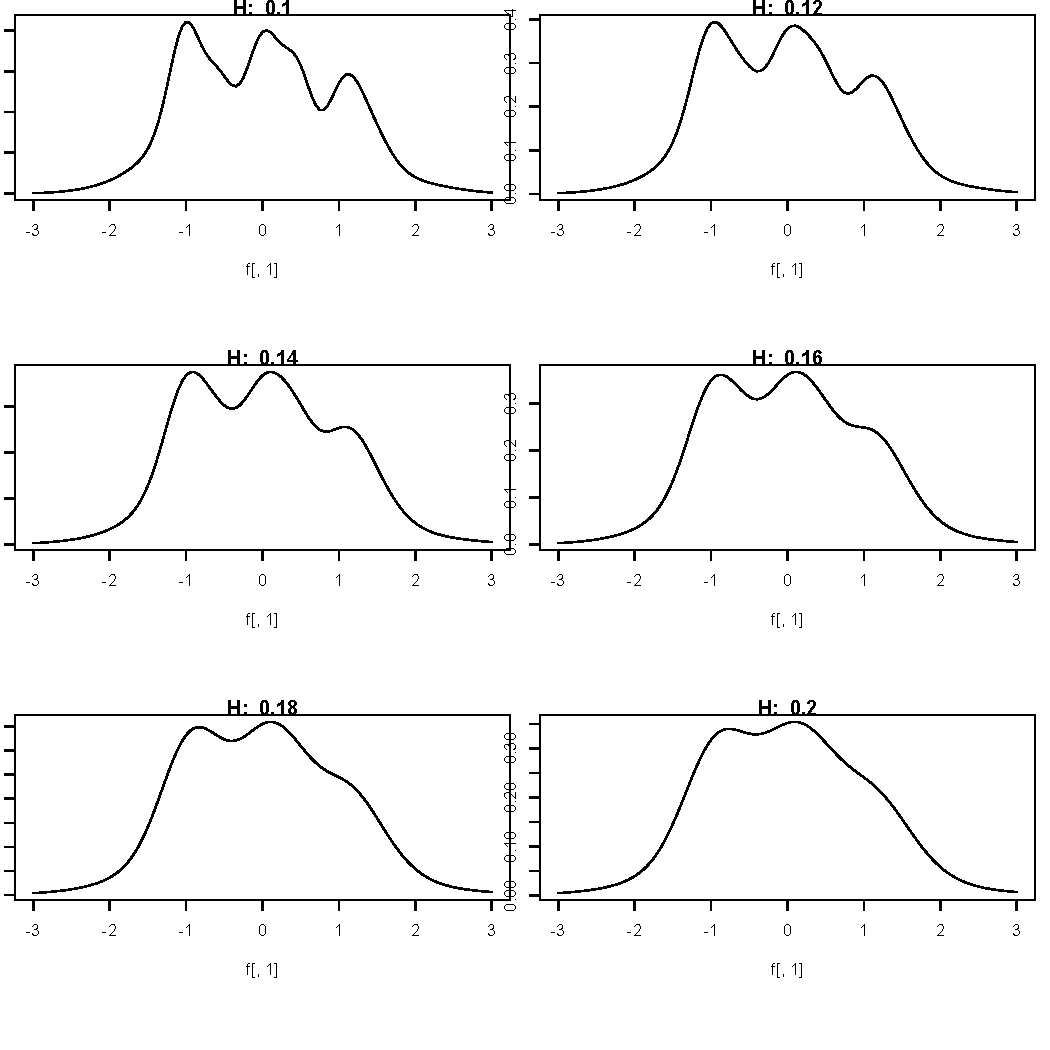
\includegraphics[width = 0.6\textwidth]{p2.pdf}
\end{figure}

Here, $h>.14$ seems to oversmooth the data, leaving $h = 0.1, 0.12, 0.14$. It appears again that $h = 0.12$ offers the best fit. This bandwidth successfully smooths out unwanted noise while identifying modes inherent in the data. To see the variable kernel estimate with $h = 0.12$ against the fixed bandwidth model, consider the figure below. 

\begin{figure}[h!]
\centering
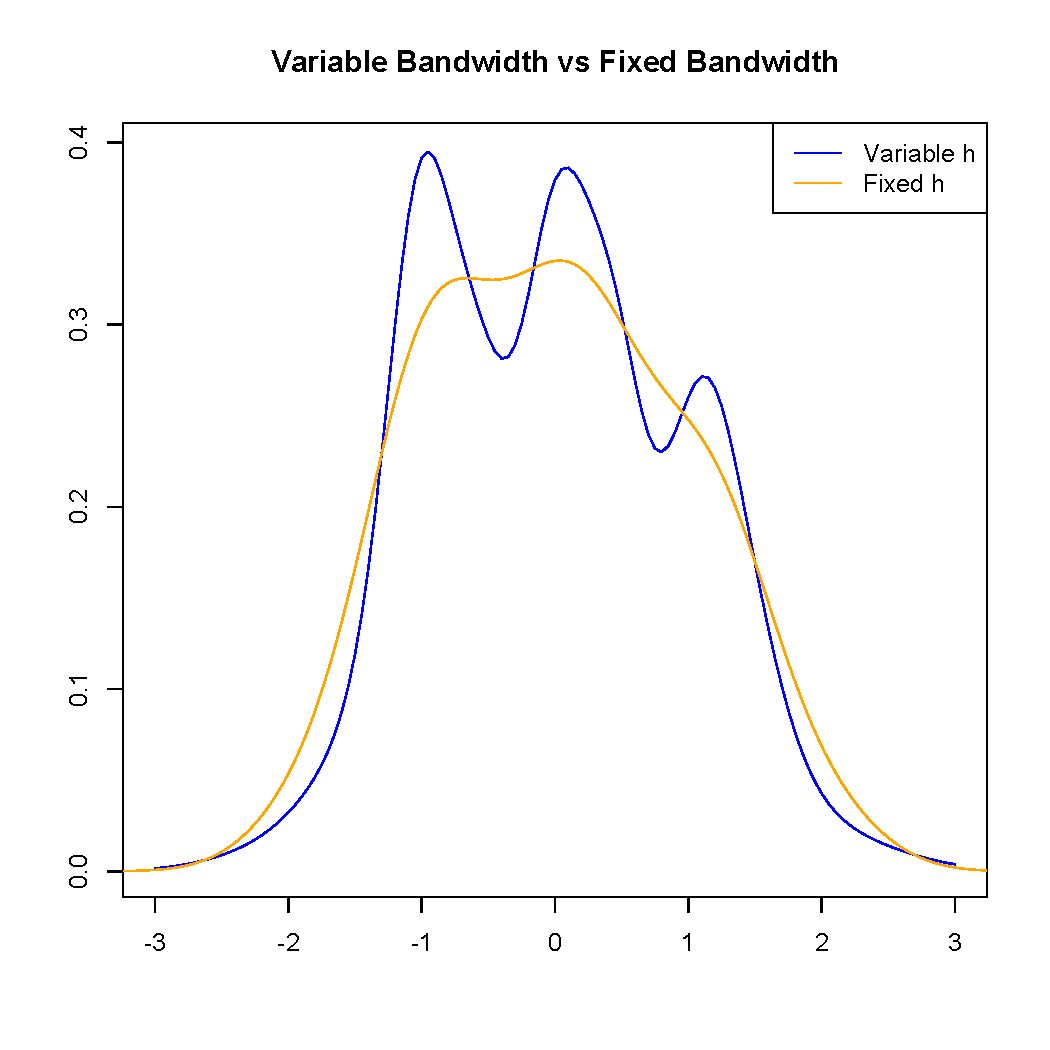
\includegraphics[width = 0.6\textwidth]{p3.pdf}
\end{figure}

Here we see that the fixed bandwidth kernel fails to find any of the modes in the distribution while the variable bandwidth manages to recover three modes. This is a drastic improvement on the global bandwidth model. 

Having attained an optimal bandwidth $h$, we now turn our attention to what affect the bandwidth and kernel choices of $\widetilde{f}$ have on our estimate of $\widehat{f}$. We consider the uniform, triangular, and Gaussian kernel as well as bandwidths of sizes of $g = 0.1, 0.25, 0.5$. To see the affect of bandwidth of $\widetilde{f}$ on $\widehat{f}$ consider the figure below. 

\begin{figure}[h!]
\centering
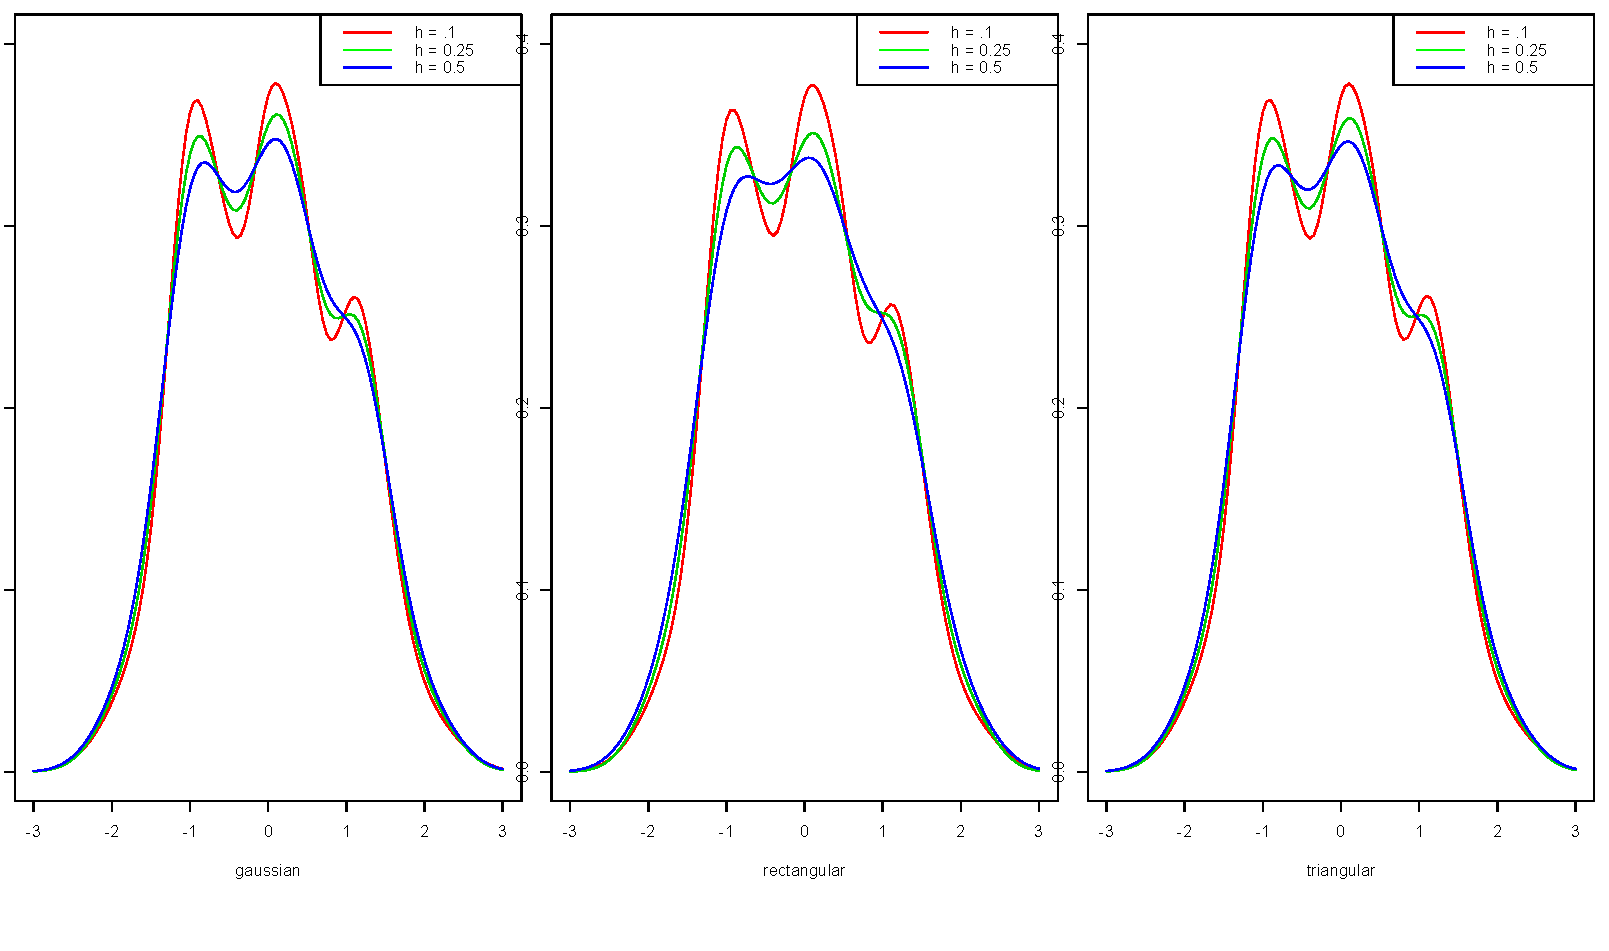
\includegraphics[width = 0.9\textwidth]{p4.pdf}
\end{figure}

Here we see that the bandwidth of $\widetilde{f}$ greatly impacts the performance of our procedure for any kernel. For higher bandwidths of $g$, we begin to remove modes in the density while lower values of $g$ we see a more modes. For the affect of the kernel on the estimation consider the figure below.
\begin{figure}[h!]
\centering
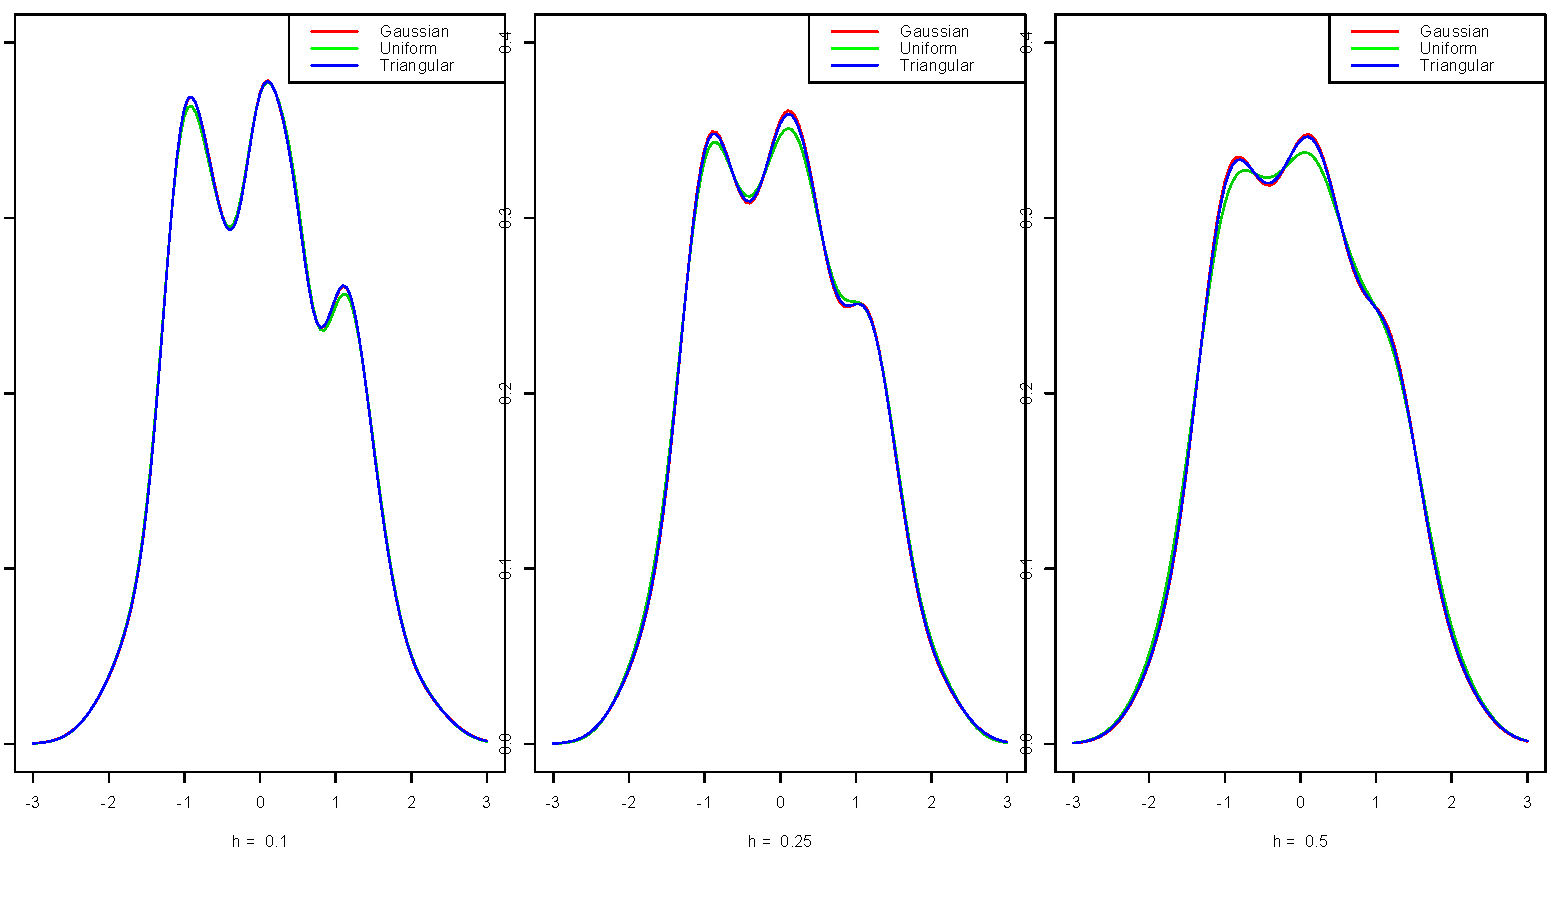
\includegraphics[width = 0.9\textwidth]{p5.pdf}
\end{figure}

For any bandwidth, it is almost impossible to distinguish between the density estimates. Perhaps the uniform kernel smooths more so than the other two methods, but the difference is negligible. For this reason, we choose to use a Gaussian kernel for $\widetilde{f}$ and focus on choosing an appropriate value of $g$. 


\item Suppose that $c_i \equiv \widetilde{f}(x_i)^{1/2}$ is constant. Then we look to use $MISE(h)$ as our decision function. We begin by finding the bias of the estimate. 

\begin{align*}
\E(\widehat{f}(x))&= \E\Big[\frac{1}{nh}\sum_{i=1}^{n}c_iK\Big(\frac{(x-x_i)c_i}{h}\Big)\Big]\\{}
&= \frac{1}{nh}\sum_{i=1}^{n}c_i\E\Big[K\Big(\frac{(x - x_i)c_i}{h}\Big)\Big]\\
&= \frac{1}{nh}\sum_{i = 1}^{n}c_i\int K\Big(\frac{(x - w)c_i}{h}\Big)f(w)dw\\
\end{align*} Now completing a change of variable for $z = \frac{(x - w)c_i}{h}$, followed by a Taylor series expansion we have 
\begin{align*}
&= \frac{1}{nh}\sum_{i = 1}^{n}c_i\int K(z)f(x - zh/c_i)\frac{h}{c_i}dz\\
&= \frac{1}{n}\sum_{i=1}^{n}\int K(z)\Big\{f(x) - f'(x)\frac{zh}{c_i} + f''(x)\frac{z^2h^2}{2c_i^2} + O(h^3)\Big\} dz\\
&= \frac{1}{n}\sum_{i=1}^{n}\bigg\{f(x)\int K(z)dz - \frac{f'(x)h}{c_i}\int zK(z)dz + f''(x)\frac{h^2}{2c_i^2}\int z^2K(z)dz + o(h^2)\bigg\}\\
&= f(x) + f''(x)h^2\mu_{2}(K)\frac{1}{2n}\sum_{i=1}^{n}c_i^{-2} + o(h^2)
\end{align*}
Using this see the bias is given by $$Bias(\widehat{f}) = f''(x)\frac{h^2}{2}\mu_{2}(K)\frac{1}{n}\sum_{i=1}^{n}c_i^{-2}$$
Now, we look to find the form of the variance of our estimator. 
\begin{align*}
Var\Big(\widehat{f}(x)\Big) &= \frac{1}{n^2h^2}\sum_{i=1}^{n}c_i^2Var\Big[K\Big(\frac{(x-x_i)c_i}{h}\Big)\Big]\\
&= \frac{1}{n^2h^2}\sum_{i=1}^{n}c_i^2\bigg[\E\Big(K\Big[\frac{(x-x_i)c_i}{h}\Big]^2\Big) - \E\Big(K\Big[\frac{(x-x_i)c_i}{h}\Big]\Big)^2\bigg]\\
&= \frac{1}{n^2h^2}\sum_{i=1}^{n}c_i^2\E\Big(K\Big[\frac{(x-x_i)c_i}{h}\Big]^2\Big) - \sum_{i=1}^{n}\bigg[\frac{c_i}{nh}\E\Big(K\Big[\frac{(x-x_i)c_i}{h}\Big]\Big)\bigg]^2\\
\end{align*}

Focusing on the first term above we have 

\begin{align*}
\frac{1}{n^2h^2}\sum_{i=1}^{n}c_i^2\E\Big(K\Big[\frac{(x-x_i)c_i}{h}\Big]^2\Big) &= \frac{1}{n^2h}\sum_{i=1}^{n}c_i^2\int K\Big(\frac{(x - w)c_i}{h}\Big)^2f(w)dw\\
&= \frac{1}{n^2h^2}\sum_{i=1}^{n}c_i^2\int K(z)^2\Big\{f(x) + O(1)\Big\}dz\\
&= \frac{1}{n^2h}\sum_{i=1}^{n}c_i\Big\{f(x)||K||_2^2 + O(1)\Big\}\\
&= \frac{f(x)||K||_2^2}{nh}\frac{1}{n}\sum_{i=1}^{n}c_i + O(1/n^2h)
\end{align*} 
Now focusing in the second term, we see that 

\begin{align*}
\sum_{i=1}^{n}\Big[\frac{c_i}{nh}\E\Big(K\Big(\frac{(x-x_i)c_i}{h}\Big)\Big)\Big]^2 &= \sum_{i=1}^{n}\Big[\frac{c_i}{nh}\int K\Big(\frac{(x-w)c_i}{h}\Big)f(w)dw\Big]^2\\
&=\sum_{i=1}^{n}\Big[\frac{1}{n}\int K(z)f(x - hz/c_i)dz\Big]^2\\
&=\sum_{i=1}^{n}\Big[\frac{1}{n}\int K(z)\Big\{f(x) + O(1)\Big\}dz\Big]^2\\
&=\sum_{i=1}^{n}\Big[\frac{1}{n}f(x) + O(1/n)\Big]^2\\
&= \frac{1}{n}f^{2}(x) + O(1/n^2) 
\end{align*}
As we argued in class, we see that this term goes to zero rapidly. Therefore, our estimate of the variance of $\hat{f}$ is given by 

$$Var(\widehat{f}(x)) = \frac{f(x)||K||_2^2}{nh}\frac{1}{n}\sum_{i=1}^{n}c_i + O(1/n^2h)$$ (Notice that if $c_i = 1$, for $i=1,2,\ldots n$, we simply get the mean and variance of the unweighted kernel). Using this we can define the MSE as 
\begin{align*}
MSE(\widehat{f}) &= \frac{f(x)||K||_2^2}{nh}\frac{1}{n}\sum_{i=1}^{n}c_i + f''(x)^2\frac{h^4}{4}\mu_{2}^2(K)\left(\frac{1}{n}\sum_{i=1}^{n}c_i^{-2}\right)^2
\end{align*}
Lastly we can find the MISE as follows 
\begin{align*}
MISE(\widehat{f}) &= \int MSE(\widehat{f})dx\\
&= \int \frac{f(x)||K||_2^2}{nh}\frac{1}{n}\sum_{i=1}^{n}c_i dx + \int f''(x)^2\frac{h^4}{4}\mu_{2}^2(K)\left(\frac{1}{n}\sum_{i=1}^{n}c_i^{-2}\right)^2 dx\\
&= \frac{||K||_2^2}{nh}\frac{1}{n}\sum_{i=1}^{n}c_i\int f(x)dx + \frac{h^4}{4}\mu_{2}^2(K)\left(\frac{1}{n}\sum_{i=1}^{n}c_i^{-2}\right)^2\int f''(x)^2 dx\\
&= \frac{||K||_2^2}{nh}\frac{1}{n}\sum_{i=1}^{n}c_i + \frac{h^4}{4}\mu_{2}^2(K)||f''||_2^2\left(\frac{1}{n}\sum_{i=1}^{n}c_i^{-2}\right)^2
\end{align*}
We now look to minimize MISE as a function of $h$. 
$$\frac{\partial}{\partial h}MISE(\widehat{f}) = -\frac{||K||_2^2}{nh^2}\frac{1}{n}\sum_{i=1}^{n}c_i + h^3\mu_2^2(K)||f''||_2^2\left(\frac{1}{n}\sum_{i=1}^{n}c_i^{-2}\right)^2 \overset{set}{=}0$$ This implies 

$$h_{MISE} = \bigg[\frac{||K||_2^2\frac{1}{n}\sum_{i=1}^{n}c_i}{\mu_2^2(K)||f''||_2^2\left(\frac{1}{n}\sum_{i=1}^{n}c_i^{-2}\right)^2}\Big]^{1/5}n^{-1/5}$$

As in the MISE for the fixed bandwidth, we require that we have some estimate of $f''$. One method was simply to refer to the normal density and calculate $||\phi||_2^2$. We can improve this estimate however. We needed an initial kernel estimate $\widetilde{f}$ is aid in our variable bandwidth procedure. In theory, this kernel should approximate the global features of $f$ and will serve as a more informative estimate of $||f''||_2^2$. Of course, we will need to estimate this value. But as we discussed in class, there are several powerful methods for this estimation procedure. During implementation, we use a helper package, \textit{kedd}, to estimate, $\widetilde{f}''$ from $\widetilde{f}$ and then carry out our own approximation of $||\widetilde{f}''||_2^2$. (Again for implementation details, see the code attached below). Using this as our plug-in estimator, our estimate of $h$ can be written as 


$$\hat{h}_{MISE} = \bigg[\frac{||K||_2^2\frac{1}{n}\sum_{i=1}^{n}c_i}{\mu_2^2(K)||\widetilde{f}''||_2^2\left(\frac{1}{n}\sum_{i=1}^{n}c_i^{-2}\right)^2}\Big]^{1/5}n^{-1/5}$$

For our sample data, we calculate that $\hat{h}_{MISE} = 0.077$ which is smaller than our original estimate of $h$ but was still considered a reasonable value after our initial grid search. The kernel density estimate given from this procedure can be seen below. 

\begin{figure}[h!]
\centering
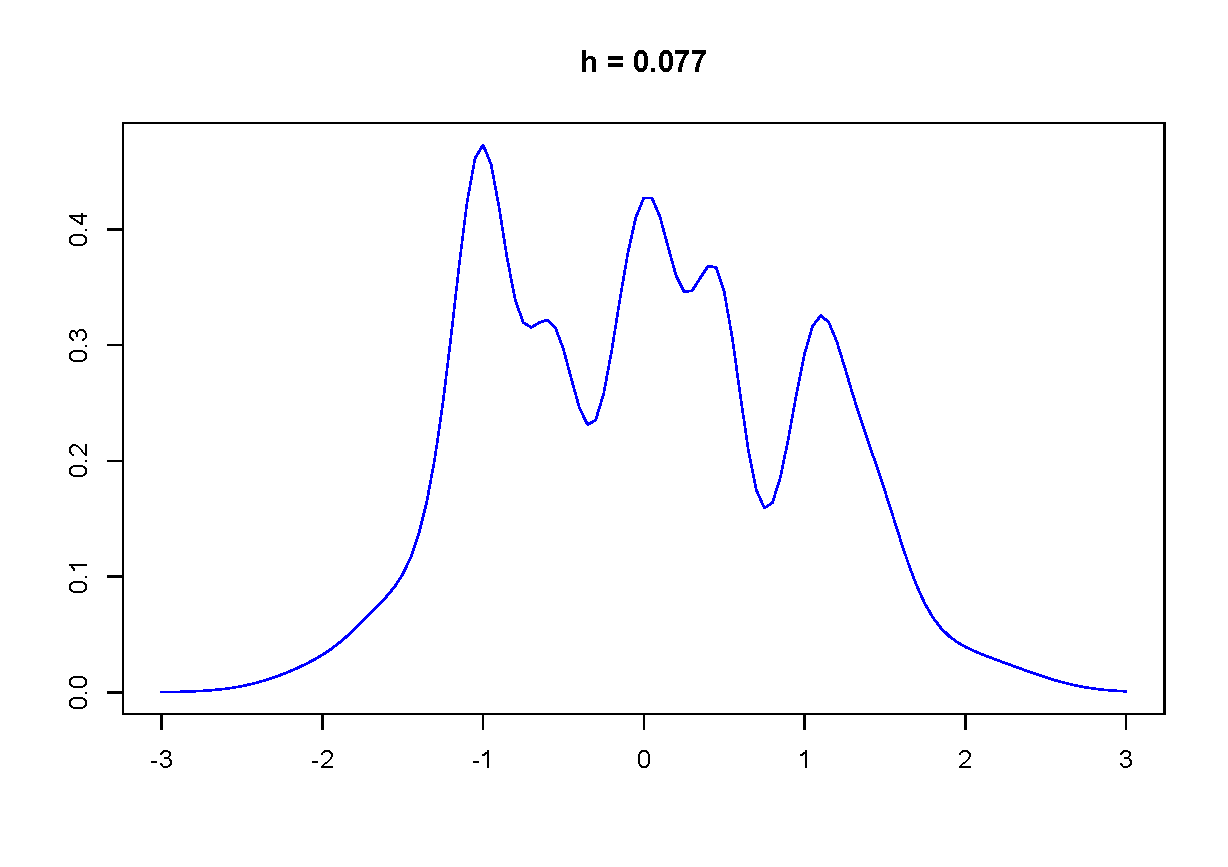
\includegraphics[width = 0.9\textwidth]{p6.pdf}
\end{figure}

This estimate appears to under smooth the data. But recall that the data we were given has four modes, not three that our initial estimate identified. Here, this kernel estimate appears to have found three, possible four modes. In any case, $\hat{h}_{MISE}$ and the variable bandwidth procedure clearly out preform the global bandwidth procedure. 

\end{enumerate}

\newpage

\item \begin{enumerate}
\item Let $\widehat{f}'$ be given by $$\widehat{f}'(x) = \frac{1}{h^2}\sum_{i=1}^{n}K'\Big(\frac{x - X_i}{h}\Big)$$ where $f$ is defined on $[0,\infty)$ and $K$ on $[-1,1]$. Suppose further that $x$ is a boundary point. That is for some $0\leq p <1$, $x = ph$. We can then calculate the expected value of this estimate near the boundary as follows. 

\begin{align*}
\E(\widehat{f}') &= \E\bigg[\frac{1}{nh^2}\sum_{i=1}^{n}K'\Big(\frac{x-X_i}{h}\Big)\bigg]\\
&= \frac{1}{h^2}\E\bigg[K'\Big(\frac{x-X}{h}\Big)\bigg]\\
&= \frac{1}{h^2}\int_{0}^{\infty}K'\Big(\frac{x - w}{h}\Big)f(w)dw\\
&=-\frac{1}{h^2}\int_{p}^{-\infty}K'(z)f(x-zh)hdz\\
\end{align*}

The the last equality was due to the substitution $z = \frac{x-w}{h}$ with $-hdz = dw$ and $w = x - zh$. Now recall that $K$ was only defined on $[-1,1]$ so $K'$ is only defined on $[-1,1]$. This gives 

\begin{align*}
&= \frac{1}{h}\int_{-\infty}^{p}K'(z)f(x-zh)dz\\
&= \frac{1}{h}\int_{-1}^{p}K'(z)f(x-zh)dz\\
&\overset{Taylor}{=}\frac{1}{h}\int_{-\infty}^{p}K'(z)\Big\{f(x)- zhf'(x) + \frac{(zh)^2}{2}f''(x) + O(h^3)\Big\}dz\\
&= \frac{f(x)}{h}\int_{-1}^{p}K'(z)dz - f'(x)\int_{-1}^{p}zK'(z)dz + \frac{hf''(x)}{2}\int_{-1}^{p}z^2K''(z)dz + O(h^2)\\
&= \frac{1}{h}a_0^1(p)f(x) - a_1^1(p)f'(x) + \frac{h}{2}a_2^1(p)f''(x) + O(h^2)
\end{align*}

\item Let $a_j^{1}(p) = \int u^jK(u)du$, $c_j^1(p)=\int u^jL(u)du$ for two kernels $K \neq L$. Then we have 
\begin{align*}
\E(c_2^1(p)\hat{f}_{K}) &= \frac{1}{h}c_2^1(p)a_0^1(p)f(x) - c_2^1(p)a_1^1(p)f'(x)+\frac{h}{2}c_2^1(p)a_2^1(p)f''(x)+O(h^2)\\
\E(a_2^1(p)\hat{f}_{L}) &= \frac{1}{h}a_2^1(p)c_0^1(p)f(x) - a_2^1(p)c_1^1(p)f'(x)+\frac{h}{2}a_2^1(p)c_2^1(p)f''(x)+O(h^2)
\end{align*}

Define $B(u) = c_2^1(p)K(u) - a_2^1(p)L(u)$. Then we have that $$\E(\widehat{f}_B(x)) = \frac{1}{h}\{a_2^1(p)c_0^1(p) - c_2^1(p)a_0^1(p)\}f(x)-\{c_2^1(p)a_1^1(p) - a_2^1(p)c_1^1(p)\}f'(x) + O(h^2)$$
Now, by letting $b_a^c(p) = a_2^1(p)c_0^1(p) - c_2^1(p)a_0^1(p)$ and $b_c^a(p) = c_2^1(p)a_1^1(p) - a_2^1(p)c_1^1(p)$ we can write 

$$\E(\widehat{f}_B(x)) = \frac{1}{h}b_a^c(p)f(x) - b_c^a(p)f'(x) + O(h^2)$$
Notice that we can repeat this exact process for two different starting kernels $K'\neq L'$ to attain that $$\E(\widehat{f}_D(x)) = \frac{1}{h}d_e^f(p)f(x) - d_f^e(p)f'(x) + O(h^2)$$ Using the kernels $B,D$ we can then remove the bias in the $f'$ term by the following weights.  

\begin{align*}
\E(d_f^e\widehat{f}_B(x)) &= \frac{1}{h}d_f^eb_a^c(p)f(x) - d_f^eb_c^a(p)f'(x) + O(h^2)\\
\E(b_c^a\widehat{f}_D(x)) &= \frac{1}{h}b_c^ad_e^f(p)f(x) - b_c^ad_e^f(p)f'(x) + O(h^2)
\end{align*}

So defining the kernel $F(u) = \frac{d_f^e(p) B(u) - b_c^a(p)D(u)}{\frac{1}{h}(d_f^eb_a^c - b_c^ad_e^f)}$ implies that $$\E(\widehat{f}_{F}(x)) = f(x) + O(h^2)$$

Therefore, we see that by weighting two kernels, we can successfully remove the $f''$ bias term and then combining a \textit{combination} of kernels, we can remove the bias of the $f'$ term. Therefore, we can remove the bias in the boundary case of $f'$ by properly weighting, then combining four separate kernels. 
\end{enumerate}


\end{enumerate}

\end{document} 

